\documentclass[a4paper, 10pt]{article}
\usepackage[brazil]{babel}
\usepackage[utf8]{inputenc}
\usepackage[T1]{fontenc}
\usepackage{ae}
\usepackage[pdftex]{graphicx}
%\pagestyle{headings}
\usepackage{indentfirst}
\graphicspath{{imagens/}}

\begin{document}
%\title{Relatório de Programação Paralela: Multiplicação de Matrizes sequencial\\}
%\author{Bernard Menezes Moreira da Costa e Thiago Figueiredo Costa}
%\date{09 de abril de 2017}
\begin{center}
{\huge Relatório de Programação Paralela: Multiplicação de Matrizes sequencial \\[7.5cm]}
{\Large Bernard Menezes Moreira da Costa\\Thiago Figueiredo Costa\\[10cm]11 de maio de 2017}
\end{center}
%\maketitle
\newpage
\section{Introdução}
O trabalho visa a aplicação de conhecimentos adquiridos na matéria de programação paralela a fim de otimizar um algoritmo de multiplicação de matrizes. Usualmente programadores recorrem a um método de multiplicação de matrizes trivial:
%FOTO
\begin{figure}[!h]
\centering
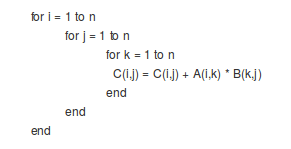
\includegraphics[scale=0.6]{pseudocodigo}
\caption{Pseudocódigo trivial de multiplicação de matriz A * B = C}
\label{Pseudocódigo}
\end{figure}

O método acima está correto, entretanto, não aproveita todo o potencial que o hardware possui, uma vez que existem diversos fatores a serem explorados pelo software. Foi fornecido pela professora do curso um de benchmark, através dele foi possível analisar o ganho computacional obtido na solução proposta pela dupla. Inicialmente o trabalho deveria ser feito forçando o compilador a evitar toda forma de vetorização através da flag "-O0". Depois deveria-se comparar o resultado com o mesmo programa vetorizado usando as flags "-O3 -ftree-vectorize -march=native -nostartfiles"  e também comparar com o programa escrito de forma paralela.

Todos os arquivos estão disponíveis em:$\linebreak$
https://github.com/SonsOfDlaiton/MatrixMultiplier,

\section{Arquivos}
A primeira parte do trabalho está na pasta "No-Vectorize" e contém todos os códigos de abordagem antiga, os testes de velocidade estão na pasta "SpeedTest", em "Old\_Code" estão os códigos de teste inicial antes de se pegar o código base da professora. Em "Auto-Vectorize" estão os arquivos usando vetorização do compilador, em "OMP" estão os arquivos usando OMP para criar o código paralelo, em "CUDA" se encontram os arquivos do protótipo para multiplicar matrizes usando CUDA. O arquivo que contém os codigos é"dgemm-dlaiton.c".

\section{Metodologia}
A princípio foi desenvolvido um speedtest, programa em C utilizado para testar quais técnicas de igual resultado são mais rápidas, a tabela a seguir representa os testes realizados:
%FOTO

Os resultados acima foram obtidos ao comparar o tempo demorado ao se realizar 10000 iterações de cada operação no mesmo computador usado para fazer o trabalho. 
Mais tarde foi realizado um brainstorm pelos integrantes da dupla visando achar maneiras para utilizar a maior parte das propriedades do hardware, nessa reunião foram discutidos quatro métodos:

O primeiro método foi chamado de método transposição implícita, o qual tenta explorar as linhas de cache do computador, nele a ordem de acesso à matriz B foi invertida de forma a realizar a multiplicação pela matriz transposta B implicitamente. Dessa maneira as linhas de cache não seriam trocadas a cada acesso de B aumentando a velocidade de acesso a valores.

O segundo método foi chamado de método de transposição explícita, nele é criada um vetor temporário BT que é preenchido de forma a ter os elementos de B porém de maneira transposta. Ele possui o mesmo princípio que motivou a realização do método de transposição implícito, porém a forma de acesso a elementos é diferente, o que foi considerado pela dupla como um fator que poderia influenciar nos resultados. Esse método foi implementado de duas maneiras diferentes, a primeira consiste em preencher a matriz BT em dois “for” exclusivos para esse preenchimento (transposição explícita simples), enquanto a segunda utiliza o “for” interno da multiplicação de matrizes para realizar posicionar os valores em BT (transposição explícita dinâmica).

O terceiro método implementado foi chamado de método de multiplicação em camadas simples, o princípio base é a disposição do resultado em camadas simples (a matriz procurada C é obtida através da disposição de resultados em uma matriz de 3 dimensões) dessa forma é possível achar o valor desejado somando as camadas. Todo esse processo foi pensado para evitar ler o resultado da matriz C durante todas as iterações do programa.
O quarto método foi chamado de método de multiplicação em camadas usando o achatamento. Esse método possui o mesmo princípio que o método de multiplicação em camadas simples, porém ele só realiza somas após fazer todas as multiplicações necessárias, de maneira a ir achatando (somando) camada por camada para obter o valor final de C.

Além desses algoritmos referenciados  acima, foi implementado o algoritmo de Strassen, o mesmo divide a multiplicação de duas matrizes em várias multiplicações de submatrizes diferentes. O algoritmo foi implementado de maneira recursiva, e segue os seguintes passos: identifica o tamanho da matriz NxN e verifica se ele é potência de dois, caso contrário ele preenche a matriz com zeros até que ela tenha essa potência. Com isso, a matriz é dividida em 4 submatrizes, após isso, ele realiza multiplicações dessa submatrizes (também pelo método de Strassen) e somas dessas matrizes de maneira que o resultado final é a matriz C procurada. A principal vantagem desse método é a sua ordem de complexidade que é O($n^{2,807}$) ao invés de O($2^{3}$) que é a ordem de complexidade do algoritmo trivial, essa vantagem é obtida através de uma outra forma de multiplicar matrizes 2x2 que usa 7 multiplicações e 17 adições ao invés das 8 multiplicações e 4 adições do método trivial. Isso só funciona considerando que a operação de multiplicação consome uma quantidade bem maior de recursos do computador do que a operação de soma.

Todos os métodos foram implementados utilizando os resultados obtidos no speedtest como base.

\newpage
\section{Resultados Computacionais}
 A maneira de analisar o ganho computacional dos métodos propostos foi medir o tempo de execução comparado a dgemm otimizada oferecida na biblioteca BLAS, em porcentagem (o quanto o método testado se aproximou da solução da biblioteca). A cada teste foram testados 26 tamanhos diferentes do tamanho N = 31, 32, 96, 127, 129, 191, 229, 255, 256, 257, 319, 320, 417, 480, 511, 512, 639, 640, 767, 768 e 769. Para cada uma existe uma porcentagem referente ao teste e o número de Mflops (Mega Flops) necessários para aquela execução em específico. 

Abaixo encontra-se a tabela de resultados com destaque para as 4 melhores porcentagens encontradas:
%FOTOS
\begin{figure}[!h]
\centering
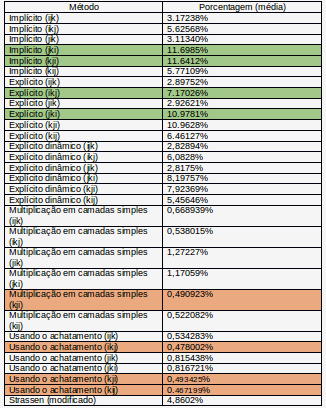
\includegraphics[scale=0.9]{resultados}
\caption{Tabela de resultados}
\label{Resultados}
\end{figure}
\vspace{1cm}

Análise gráfica por métodos:
%FOTOS
\begin{figure}[!h]
\centering
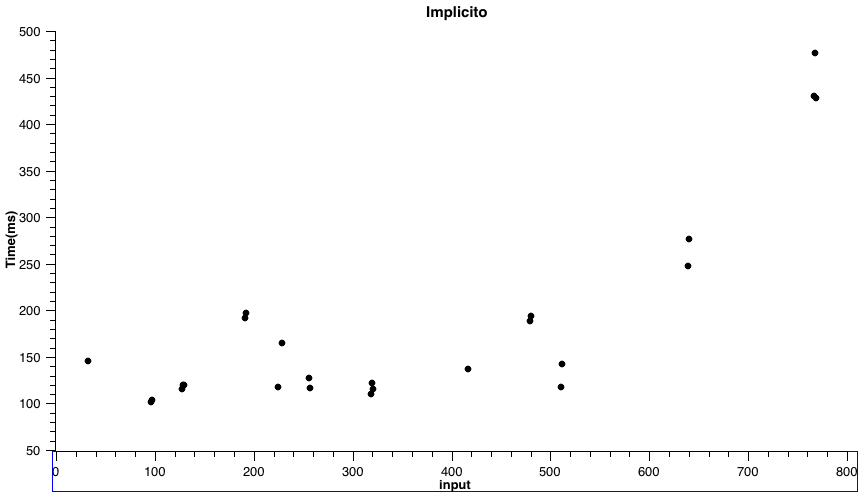
\includegraphics[scale=0.35]{implicito}
\caption{Gráfico do método implícito}
\label{Gráfico implícito}
\end{figure}
\vspace{3cm}
\begin{figure}[!h]
\centering
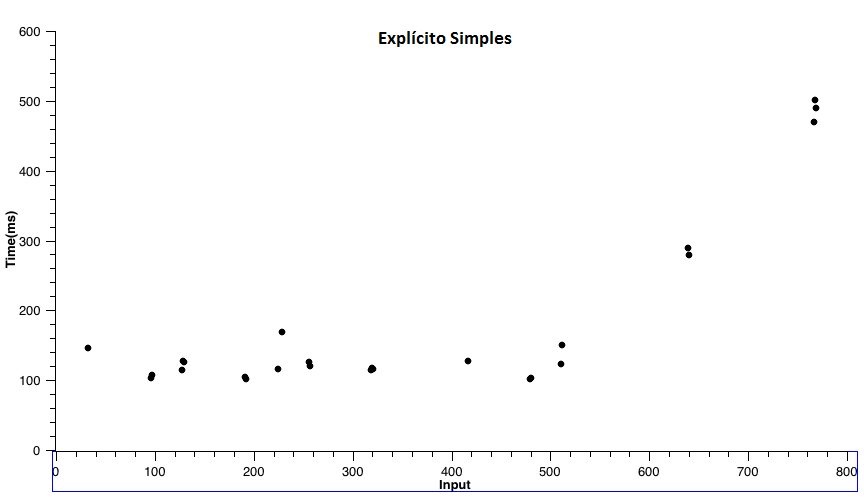
\includegraphics[scale=0.35]{explicito_simples}
\caption{Gráfico do método explícito simples}
\label{Gráfico explícito simples}
\end{figure}
\newpage
\begin{figure}[!h]
\centering
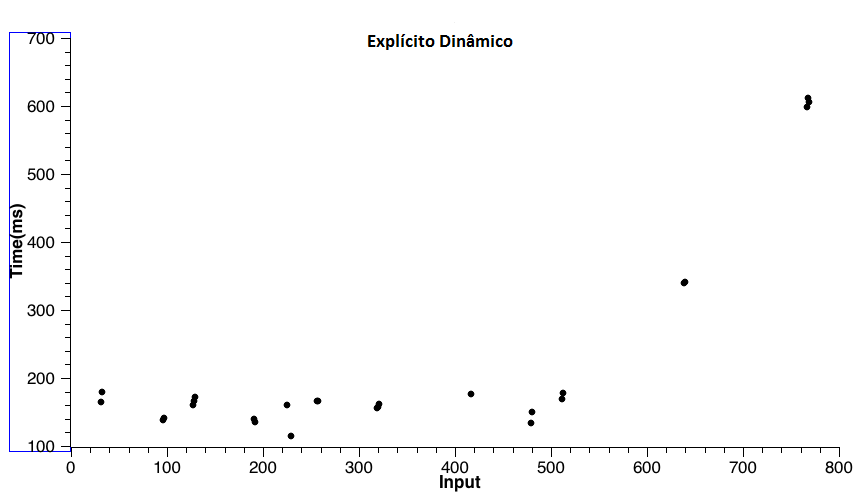
\includegraphics[scale=0.35]{explicito_dinamico}
\caption{Gráfico do método explícito dinâmico}
\label{Gráfico explícito dinâmico}
\end{figure}
\vspace{3cm}
\begin{figure}[!h]
\centering
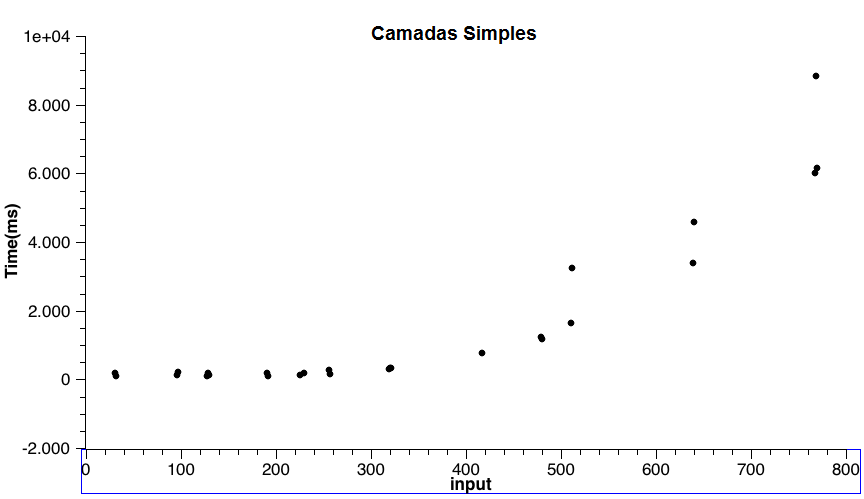
\includegraphics[scale=0.35]{camadas_simples}
\caption{Gráfico do método de multiplicação em camadas simples}
\label{Gráfico camadas simples}
\end{figure}
\newpage
\begin{figure}[!h]
\centering
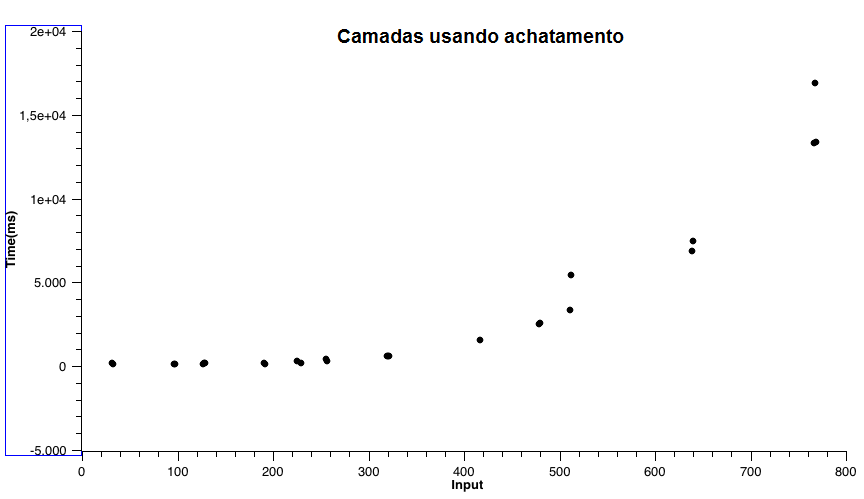
\includegraphics[scale=0.35]{camadas_achatamento}
\caption{Gráfico do método de multiplicação em camadas usando achatamento}
\label{Gráfico camadas achatando}
\end{figure}
\vspace{3cm}
\begin{figure}[!h]
\centering
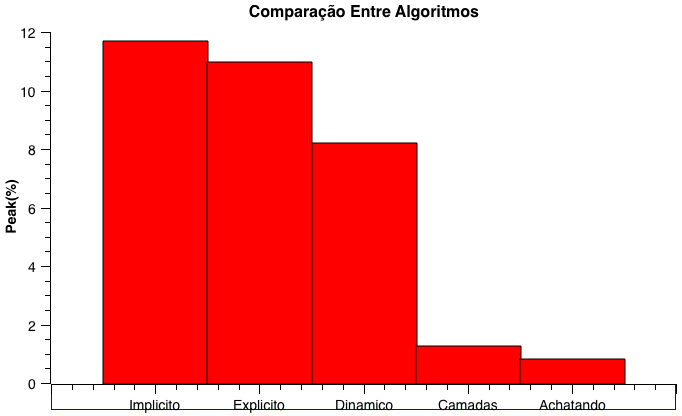
\includegraphics[scale=0.5]{comparacao_algoritmos}
\caption{Gráfico comparativo dos métodos}
\label{Gráfico comparativo}
\end{figure}
\newpage
\begin{figure}[!h]
\centering
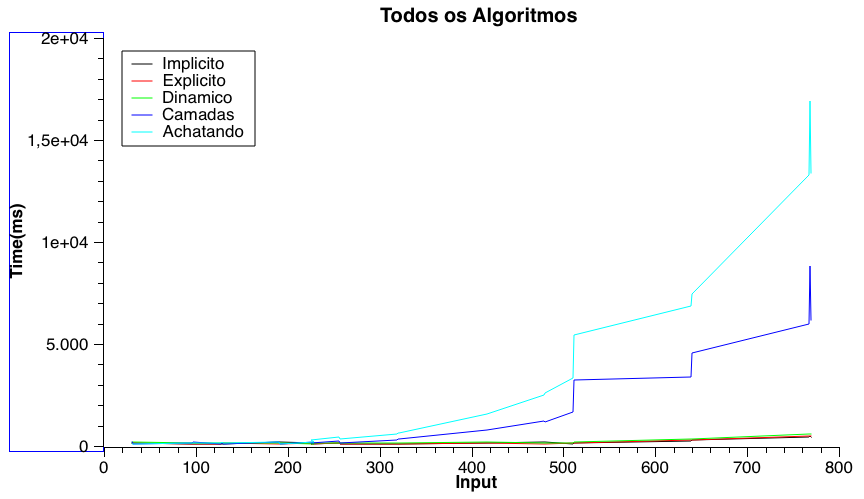
\includegraphics[scale=0.35]{todos_algoritmos}
\caption{Gráfico de desempenho de todos os algoritmos}
\label{Gráfico de todos algoritmos}
\end{figure}

Análises por métodos:

\begin{itemize}
\item Implícito: O método apresentou as duas melhores porcentagens, é possível enxergar uma melhora considerável ao alterar a ordem dos índices que acessaram as posições na matriz. Isso ocorre de acordo com cada arquitetura, uma vez que existem diversas configurações de cache. Foi possível obter o ganho de 8,5851\% ao mudar da ordem (jik) para (jki), ou seja, uma simples troca de ordem entre “i” e “k” promoveu uma alteração significativa.

\item Explícito: O método apresentou o terceiro e o quarto melhor resultado, da mesma forma que o método implícito a ordem dos índices teve uma influência considerável nos resultados. Reforçando que para a arquitetura usada a melhor ordem de índices é (jki), que teve um ganho de 8,08058\% para a pior porcentagem (ijk).

\item Camadas simples: O método não foi eficiente ao ser comparado com os demais, atingindo no máximo 1,27227\%, é de se pensar que as barreiras condicionais existentes nele podem torna-lo lento. Além disso, o fato desse método não ser otimizado para usufruir das linhas de cache pode ter influenciado no resultado obtido. Obteve a pior medida, que foi de 0,490923\%.

\item Camadas usando achatamento: O método, assim como o de multiplicação em camadas simples, não se mostrou muito eficiente para resolver o problema em questão. Mais uma vez o fato do método não ser otimizado para usufruir das linhas de cache influenciou negativamente no resultado.

\item Strassen: O método achou o resultado desejado, porém com tamanhos acima 319 o algoritmo é totalmente inviável de ser executado, suas chamadas de recursão são tantas que acabam por ocupar grande parte da memória do computador chegando a travá-lo. Como não foi possível executar para todos os tamanhos nenhuma porcentagem média foi gerada, e por isso nenhum gráfico foi gerado. Após discussão conjunta a dupla decidiu reduzir o número de recursões, de  maneira proporcional ao tamanho de cache, quando uma das chamadas da funções passar como parâmetro uma matriz NxN a qual o custo de cálculo com o algoritmo implícito seja pequeno a chamada das multiplicações dessa submatriz passa a ocorrer com o método implícito, dando fim à recursividade desnecessária. Dessa maneira foi obtida uma porcentagem nova de 4,8602\%.
\end{itemize}

Após a plotagem dos gráficos, foi analisado o desempenho de cada algoritmo em relação o tamanho de entrada. Foi procurado métodos que fossem mais eficientes com tamanho de entradas grandes, médios e pequenos, a ideia era que se fossem encontrados métodos ótimos diferentes para cada intervalo definido, o algoritmo a ser entregue no trabalho seria dependente do tamanho de entrada. Entretanto os resultados obtidos foram de certa forma constantes, por exemplo, o método mais eficiente testado teve os melhores resultados em todos os intervalos do tamanho de entrada.

\newpage
\section{Vetorização}
\subsection{Auto-vetorização}
Ao usar o código implicito permitindo sua vetorização obtivemos um resultado bem melhor, de 25\%, que chega a ser aproximadamente 2,3 vezes mais rápido que o código não vetorizado.
\subsection{Open MP}
Ao fazer um código usando open MP obtivemos um resultado de 7\%, que não foi satisfatório pois ficou inferior às outras abordagens.

\section{Conclusões}
Através das análises de resultados obtidos ficou claro a importância de considerar o cache ao implementar um algoritmo que tenha eficiência máxima. Todos os métodos que não levaram em consideração esse fato obtiveram resultados muito inferiores aos quais desfrutaram dessa memória. Ao tentar executar o algoritmo em outro computador foi possível perceber o quanto a arquitetura e as configurações de uma máquina interferem nos resultados dos testes, o que demonstra o quão essencial é manter as análises em uma situação específica de hardware.

Algumas alterações realizadas no código em alto nível aparentam ser mais eficientes, porém na prática não são. A implementação do método explícito dinâmico é um exemplo para essa afirmação, ao evitar a utilização de duas sequências de “for” no escopo da função era de se esperar que o tempo de execução reduzisse e consequentemente a porcentagem medida aumentasse. O contrário ocorreu, o que demonstra o quão difícil é realizar previsões quando os fenômenos de baixo nível se mostram tão essenciais para resolver um problema.

A principal conclusão permitida pela realização do trabalho foi a confirmação na prática da seguinte fórmula:
%FOTO
\begin{figure}[!h]
\centering
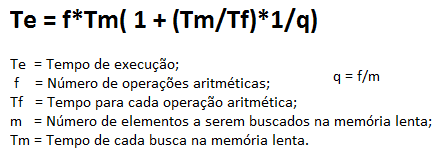
\includegraphics[scale=0.7]{formula}
\caption{Fórmula do tempo de execução de um algoritmo}
\label{Fórmula}
\end{figure}

De acordo com ela, devemos reduzir ao máximo o termo “1/q” para obtermos o melhor tempo de execução possível, para isso resta aumentar o número de operações aritméticas e reduzir os acessos à memória lenta. Os métodos que buscaram otimizar o uso da memória rápida (explícito e implícito), e consequentemente, reduziram acessos à memória lenta obtiveram os melhores resultados. Já os métodos mais lentos (multiplicação em camadas simples e usando achatamento) aumentaram o número de operações aritméticas, em contrapartida, aumentaram acessos à memória lenta o que acabou por inibir o ganho computacional.

Os resultados não foram satisfatorios pois, embora o valores obtidos tivessem sido acima do esperado para um código não vetorizado, estávamos usando o makefile que foi disponibilizado com a flag -O1 crendo que não haveria vetorização e o certo deveria ser -O0, ao perceber isso, vimos que nosso melhor código com a flag certa reduziu seu resultado para 4\%, um resultado péssimo. Por usar o ambiente incorreto durante todo o trabalho não foi possível desenvolver um bom algoritmo para multiplicar matrizes sem vetorizar.


\end{document}